% !TEX root = ../main.tex

\begin{table}[t]
\centering
\begin{tabular}{|p{2.5cm}|p{7cm}|p{2.5cm}|}
\hline

$\Sigma$-Protocols 
& The first proofs of solvency are based on $\Sigma$-Protocols which work on standard elliptic curves like \secp but are not succinct (linear proof space, linear verifier time, heavy constants). 
& Provisions~\cite{provisions} \\ \hline

Inner-product arguments 
& Protocols like bulletproofs work on standard elliptic curves like \secp and can reduce some sub-routines (e.g., range arguments) to constant space and logarithmic verifier time. 
& Bulletproofs~\cite{bulletproofs} \\ \hline

Liabilities only 
& As it is the asset-side of solvency that ties the protocol to standard elliptic curves like \secp, proving only the liability side can be done in any cryptographic setting. 
& ZeroLedge~\cite{zeroledge}, DAPOL+~\cite{dapol}, SSVT-based~\cite{spp}, Notus~\cite{notus}, SafeCex\tablefootnote{V. Buterin, ``Having a safe CEX: proof of solvency and beyond,'' \href{https://web.archive.org/web/20230919210728/https://vitalik.ca/general/2022/11/19/proof_of_solvency.html}{vitalik.ca}, 2022} \\ \hline

Publish assets 
& A trivial proof of assets is one that is not zero-knowledge. An exchange could reveal all its addresses and prove ownership by signing a proof-specific message from each address.
& Summa\tablefootnote{\url{https://summa.gitbook.io/summa}} \\ \hline

Circuit-level 
& A general zk-snark can implement any arithmetic circuit, including \secp operations, which offers a proof of constant size and constant verifier time. 
& IZPR~\cite{izpr}, Proven.tools\tablefootnote{\url{https://www.proven.tools/}} \\ \hline

Custom blockchain 
& If new blockchains are deployed, they could use digital signatures over pairing-friendly curves. 
& Mina\tablefootnote{\url{https://minaprotocol.com/}} \\ \hline

Mapping between groups 
& If \secp values can be mapped to a pairing-friendly group, Poly-IOP arguments can potentially reduce the rest of the proof to constant size and constant verifier time. 
& COPZ~\cite{chase22}, \Sys \\ \hline

\end{tabular}
\caption{How to deal with the fact that Bitcoin and Ethereum use \secp digital signatures when trying to make a succinct proof of solvency.\label{tab:rb1}}
\end{table}

%\begin{figure}[t]
%\centering
%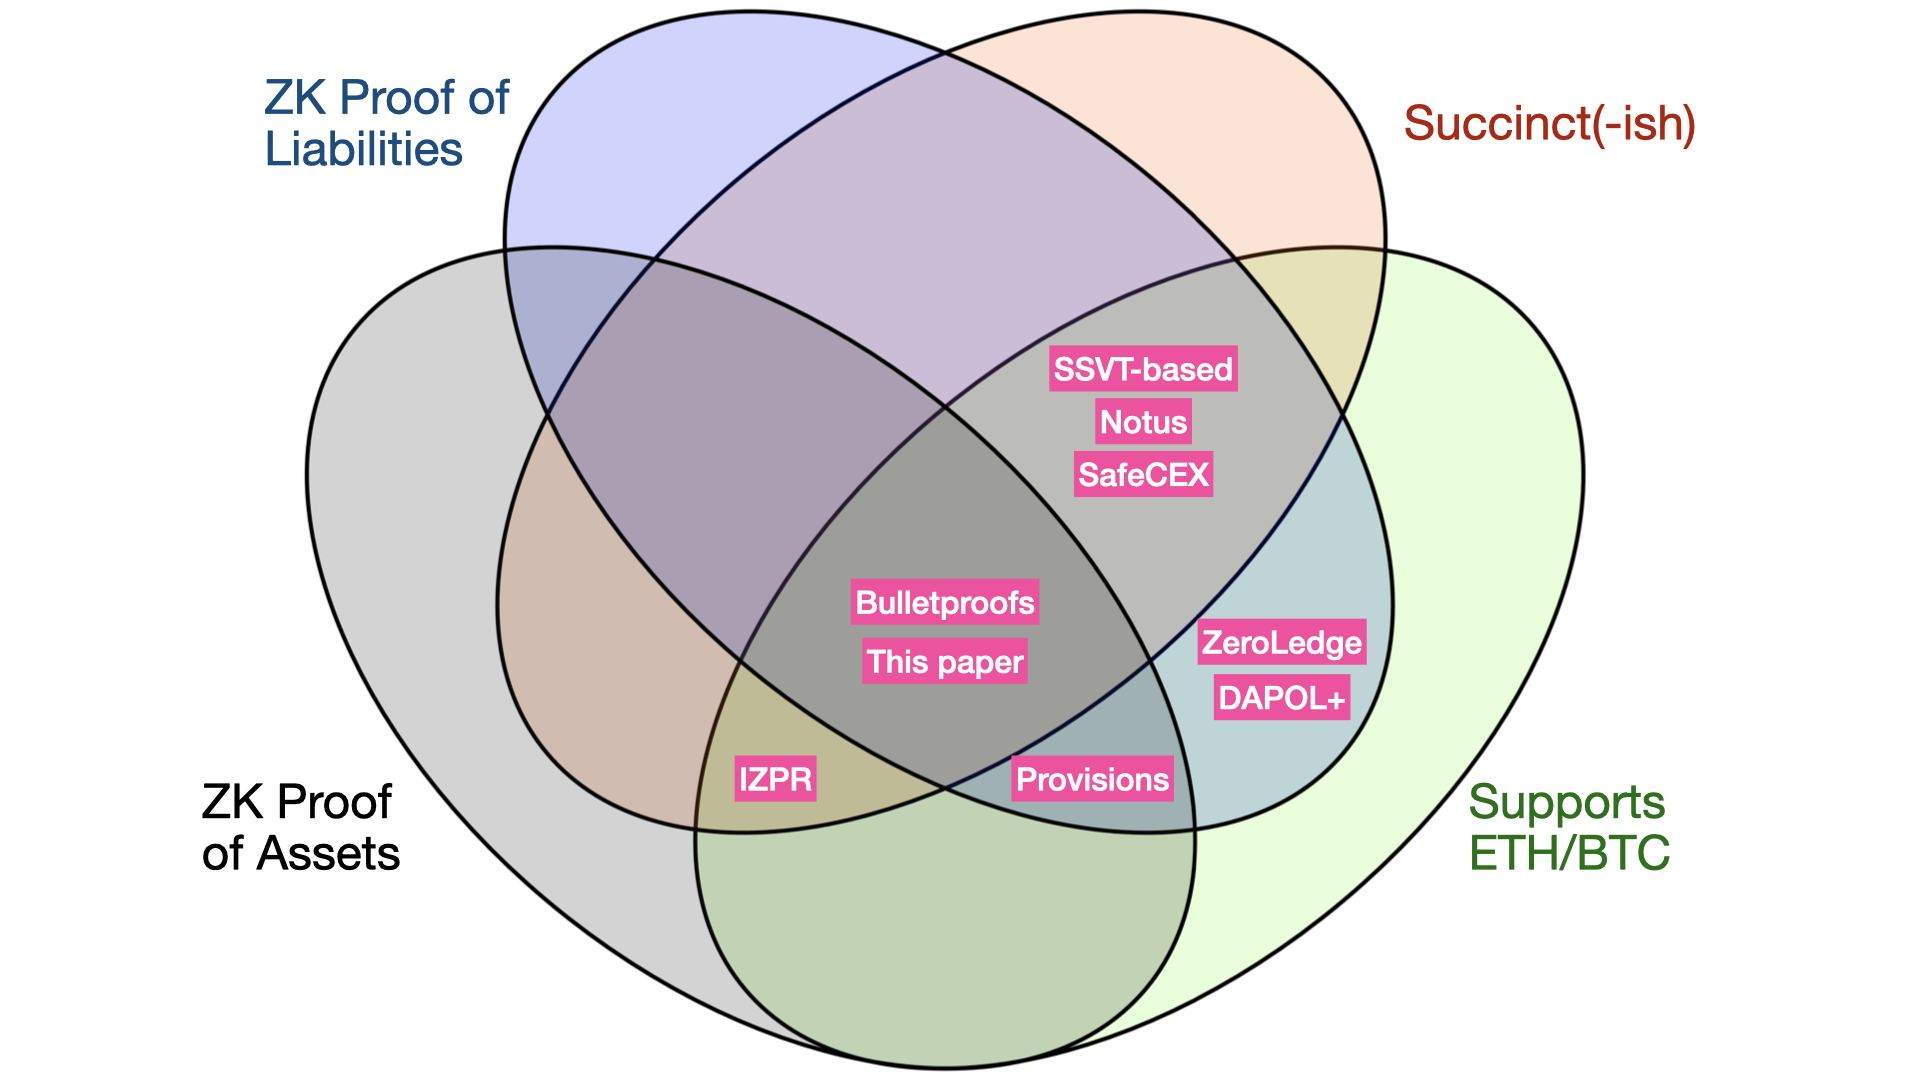
\includegraphics[width=0.8\textwidth]{figures/venn.png}
%\caption{default. \label{default}}
%\end{figure}